\begin{figure}
	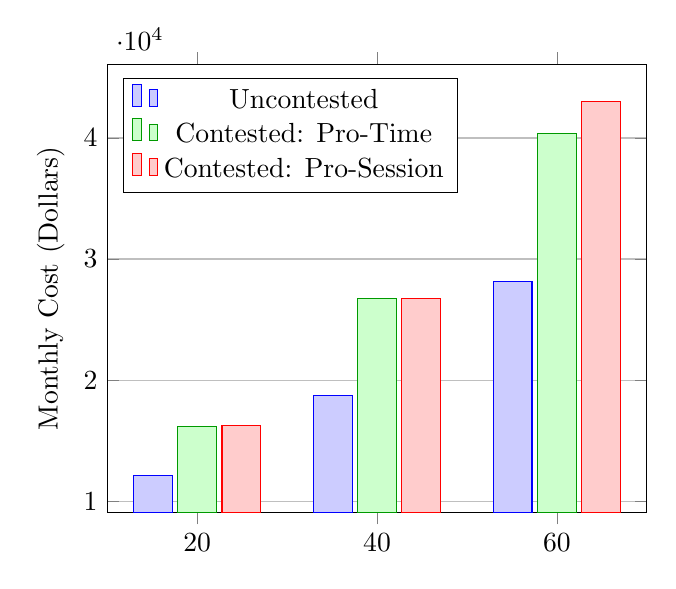
\begin{tikzpicture}
		\begin{axis}[ybar, bar width=14pt, xmin=10, xmax=70, xtick={20, 40, 60},ymajorgrids=true, ylabel={Monthly Cost (Dollars)}, legend pos=north west]
			\addplot[fill=blue!20, draw=blue] coordinates {
				(20, 12150.65)
				(40, 18745.58)
				(60, 28166.09)
			};
			\addplot[fill=green!20, draw=black!40!green] coordinates {
				(20, 16183.79)
				(40, 26738.71)
				(60, 40405.72)
			};
			\addplot[fill=red!20, draw=red] coordinates {
				(20, 16256.21)
				(40, 26738.71)
				(60, 43007.78)
			};
		\legend{Uncontested, Contested: Pro-Time, Contested: Pro-Session};
		\end{axis}
	\end{tikzpicture}
	\caption{Comparison of Monthly Costs}
	\label{fig:results:contestedVsUncontestedPrice}
\end{figure}


